% =====================================================================================
%  DocROI-Former-QDCT -- research paper (draft for supervisor review)
%  Build:  tectonic DocROI-Former-QDCT_paper.tex     (or: pdflatex, run twice)
%  Figures are read from ../docs/ (see \graphicspath below).
% =====================================================================================
\documentclass[11pt,a4paper]{article}

\usepackage[margin=2.4cm]{geometry}
\usepackage[T1]{fontenc}
\usepackage{lmodern}
\usepackage{microtype}
\usepackage{amsmath,amssymb}
\usepackage{booktabs}
\usepackage{tabularx}
\usepackage{array}
\usepackage{multirow}
\usepackage{xcolor}
\usepackage{graphicx}
\usepackage{enumitem}
\usepackage[font=small,labelfont=bf]{caption}
\usepackage{tikz}
\usetikzlibrary{positioning,arrows.meta,fit,calc}
\usepackage[colorlinks=true,linkcolor=blue!50!black,citecolor=blue!50!black,urlcolor=blue!50!black]{hyperref}

\graphicspath{{../docs/}}
\newcommand{\ours}{DocROI-Former-QDCT}
\newcommand{\R}{\mathbb{R}}
\newcommand{\best}[1]{\textbf{#1}}
\setlist{itemsep=2pt,topsep=3pt}
\renewcommand{\arraystretch}{1.12}

\title{{\LARGE\textbf{\ours}}\\[8pt]
{\Large\textbf{Entity-Gated Fusion of RGB, Forensic-Residual and Quantised-DCT Evidence
for Tampered-Text Localisation in Document Images}}}
\author{Shivendra Pratap Singh}
\date{Draft for supervisor review \quad$\cdot$\quad 26 November 2026}

\begin{document}
\maketitle

% =====================================================================================
\begin{abstract}
\noindent
Text in document images can be altered so that the change is almost invisible, and the image
is then usually recompressed when it is shared, which erases many forensic traces. We present
\ours, a 43.9M-parameter dual-stream network for pixel-level localisation of tampered text.
An ImageNet-pretrained PVTv2-B2 encoder reads the image, and a forensic stream combines
Bayar and SRM residuals with a quantised JPEG-DCT branch that recomputes the exact coefficient
lattice of the final JPEG and is conditioned on its quantisation table. The two streams are
fused at four scales by cross-attention whose keys are restricted to document content by a
label-free entity router and stabilised by QK-normalisation, and the result is decoded by a
progressive guided-upsampling head. The model is trained only on the DocTamper training set
and was evaluated exactly once under the official DTD protocol (grayscale, one to three JPEG
rounds with DTD's per-image quality tables, minimum quality 75, all 50{,}000 test images,
fixed threshold 0.5). It reaches F1 = 78.1 / 81.5 / 72.3 and tampered-class IoU = 77.3 /
59.0 / 60.3 on TestingSet / FCD / SCD. On the cross-domain FCD split it ties ADCD-Net and is
within 0.1 F1 of DTD with two-thirds of DTD's parameters; on TestingSet and SCD it is 1--3 F1
below both, and it is well below FFDN. Error analysis shows that the remaining gap comes almost
entirely from edits covering less than 1\% of the image. We report an independent audit of the
evaluation records and state which claims still require ablation.
\end{abstract}

% =====================================================================================
\section{Introduction}\label{sec:intro}

Contracts, invoices, certificates and identity or financial documents are routinely exchanged
as scans or photographs. Changing a handful of characters, such as a date, an amount or a name,
is often enough to change the meaning of such a document, and current editing tools make these
changes hard to see. Localising tampered text at the pixel level is therefore a core task of
document forensics.

The task differs from manipulation localisation in natural images in three ways.
\begin{enumerate}
  \item \textbf{The regions are tiny and thin.} An edit is frequently a single character. On the
        DocTamper TestingSet, 62\% of the images have a tampered area below 1\% of the image
        (Section~\ref{sec:analysis}).
  \item \textbf{Most pixels are blank paper.} There, high-pass forensic residuals are dominated by
        acquisition noise (scanner noise, paper texture, folds, glare) that has nothing to do
        with tampering, while the tampering itself happens on content.
  \item \textbf{Images are recompressed.} Shared documents are typically re-saved as JPEG, often
        several times. This blurs pixel-domain traces; the traces that survive live in the
        integer lattice of the quantised DCT coefficients, and their meaning depends on the
        compression strength.
\end{enumerate}

The DocTamper benchmark~\cite{dtd} formalises this setting with 120{,}000 training images,
an in-domain test set (TestingSet, 30{,}000 images) and two cross-domain test sets (FCD,
2{,}000; SCD, 18{,}000). Its evaluation protocol converts every test image to grayscale and
JPEG-compresses it one to three times with fixed per-image quality factors. Recent methods
evaluated under this protocol include DTD~\cite{dtd}, FFDN~\cite{ffdn} and
ADCD-Net~\cite{adcd}.

\paragraph{Approach.} \ours\ treats the RGB appearance of the document and its forensic
evidence as two streams and lets the RGB stream \emph{query} the forensic stream, but only at
document content. A light router, trained without entity labels, separates content (text,
photos, codes, seals) from paper; it attenuates forensic features on paper and masks
paper tokens out of the cross-attention keys. The forensic stream contains, besides
Bayar~\cite{bayar} and SRM~\cite{srm} residuals, an exact quantised-DCT branch conditioned on
the JPEG quantisation table. A progressive decoder recovers thin regions at full resolution
with residual-guided edge refinement.

\paragraph{Evaluation discipline.} Evaluation details change conclusions. An earlier model of
ours, evaluated on \emph{uncompressed} test images with a per-image metric, appeared to exceed
the state of the art (80.7 F1 on TestingSet); under the official protocol the same model scores
56.9. Every number in this paper therefore comes from a single evaluation, under the official
protocol, of a checkpoint selected on held-out \emph{training} data. The evaluation records
are released per image and fingerprinted, and Section~\ref{sec:audit} reports an independent
audit of them.

\paragraph{Contributions.}
\begin{enumerate}[label=(\arabic*)]
  \item \textbf{Label-free entity-gated forensic fusion (N1).} A document-entity router,
        trained without entity labels, gates both the forensic features and the keys of an
        RGB$\rightarrow$forensic cross-attention, so that forensic evidence is read only from
        document content.
  \item \textbf{Quantisation-table-conditioned DCT injection (N2).} Exact quantised
        coefficients of the final JPEG, computed in fp32 even under bf16 training, are embedded,
        FiLM-conditioned on $\log Q$ and injected into the residual pyramid at strides 8 and 4
        (0.52M parameters).
  \item \textbf{Stabilised cross-modal attention (N3).} We diagnose a divergence caused by
        attention-logit growth at the stages without key normalisation and remove it with
        QK-normalisation.
  \item \textbf{Thin-region decoding and typography consistency (N4, N5).} A progressive guided
        upsampling decoder with native-resolution SRM edge gating, and an intra-document
        font-consistency objective used only in training.
  \item \textbf{Leak-proof training and an auditable evaluation.} Training degradations follow
        the test protocol's family without reading its tables; selection uses held-out training
        images; the selected checkpoint is evaluated once with SHA-256 fingerprints and 50{,}000
        per-image records, which we audit.
\end{enumerate}
The system result supports the combination of N1--N5. The individual contributions of N1, N2,
N4 and N5 are \emph{not yet} isolated by ablation (Section~\ref{sec:limits}).

% =====================================================================================
\section{Related work}\label{sec:related}

\paragraph{Image manipulation localisation.} General-purpose detectors learn traces of
editing from natural images. ManTra-Net~\cite{mantra} learns manipulation traces and detects
local anomalies; MVSS-Net~\cite{mvss} combines edge and noise views with multi-scale
supervision; PSCC-Net~\cite{pscc} uses progressive spatio-channel correlation;
CAT-Net~\cite{catnet} adds a DCT stream that learns JPEG compression artifacts from one-hot
quantised coefficients; and TruFor~\cite{trufor} fuses RGB with a learned noise-sensitive
fingerprint and predicts a reliability map. Semantic-segmentation transformers such as
Swin~\cite{swin} and BEiT~\cite{beit} with an UPerNet head~\cite{upernet} are also used as
baselines. Under the DocTamper protocol these methods trail document-specific models by a
wide margin (Table~\ref{tab:f1}).

\paragraph{Document tampering.} DTD~\cite{dtd} introduced the DocTamper dataset together with
a model that adds a frequency perception head on DCT coefficients and a multi-view iterative
decoder to a visual encoder, trained with a curriculum (CLTD) that progressively lowers the
compression quality. FFDN~\cite{ffdn} improves tampered-text detection through frequency
feature fusion and decomposition on a ConvNeXtV2-B backbone (140M parameters).
ADCD-Net~\cite{adcd} weights DCT features adaptively by a predicted alignment score and
disentangles content hierarchically to reduce the bias between text and background, with
23M parameters. Our router (N1) addresses the same text--background disparity as ADCD-Net, but
by routing: it gates the forensic features and the attention keys rather than disentangling
content features.

\paragraph{Building blocks.} Our RGB encoder is PVTv2~\cite{pvtv2}, whose spatial-reduction
attention we reuse for cross-modal fusion. Forensic residuals come from the constrained
convolution of Bayar and Stamm~\cite{bayar} and fixed SRM filters~\cite{srm}. The one-hot
encoding of quantised coefficients follows CAT-Net~\cite{catnet} and DTD~\cite{dtd};
conditioning uses FiLM~\cite{film}; QK-normalisation is from Dehghani
\emph{et al.}~\cite{qknorm}. The training objective uses focal~\cite{focal}, Dice, boundary
\cite{boundary} and InfoNCE~\cite{infonce} terms.

% =====================================================================================
\section{Method}\label{sec:method}

\begin{figure}[t]
\centering
\resizebox{\textwidth}{!}{%
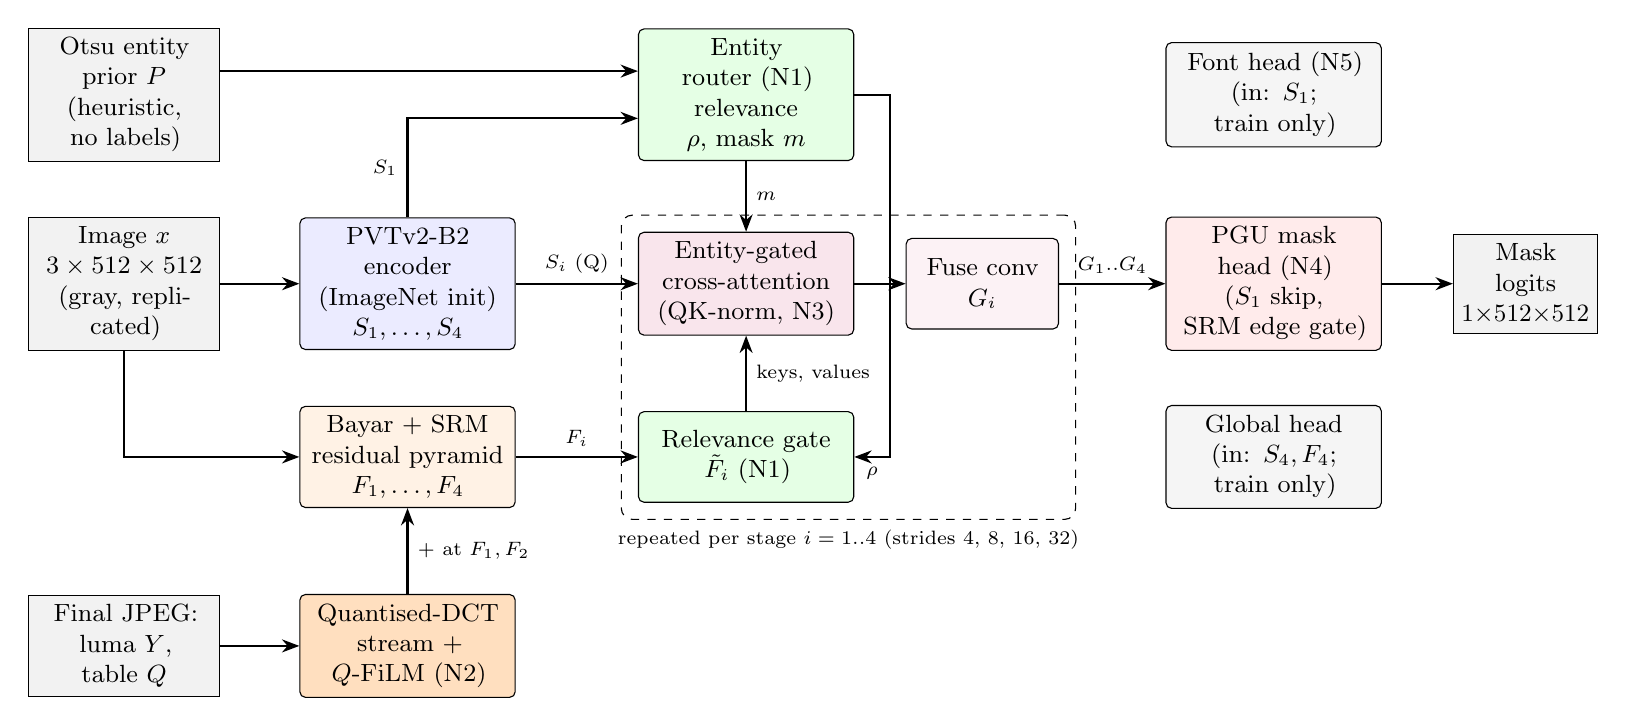
\begin{tikzpicture}[
  font=\small,
  blk/.style={draw, rounded corners=2pt, align=center, minimum height=1.15cm, text width=2.5cm, fill=#1},
  blk/.default={white},
  io/.style={draw, align=center, minimum height=1.0cm, text width=2.2cm, fill=gray!10},
  arr/.style={-{Stealth[length=2.2mm]}, thick},
  lbl/.style={font=\scriptsize, midway}
]
\node[io]  (prior) at (0, 4.6)  {Otsu entity prior $P$\\(heuristic, no labels)};
\node[io]  (img)   at (0, 2.2)  {Image $x$\\$3\times512\times512$\\(gray, replicated)};
\node[io]  (jpeg)  at (0,-2.4)  {Final JPEG:\\luma $Y$, table $Q$};
\node[blk=blue!8]   (pvt)  at (3.6, 2.2)  {PVTv2-B2 encoder\\(ImageNet init)\\$S_1,\dots,S_4$};
\node[blk=orange!10](res)  at (3.6, 0.0)  {Bayar + SRM\\residual pyramid\\$F_1,\dots,F_4$};
\node[blk=orange!25](qdct) at (3.6,-2.4)  {Quantised-DCT\\stream + $Q$-FiLM (N2)};
\node[blk=green!10] (router) at (7.9, 4.6) {Entity router (N1)\\relevance $\rho$, mask $m$};
\node[blk=green!10] (gate)   at (7.9, 0.0) {Relevance gate\\$\tilde F_i$ (N1)};
\node[blk=purple!10](xattn)  at (7.9, 2.2) {Entity-gated\\cross-attention\\(QK-norm, N3)};
\node[blk=purple!5, text width=1.7cm] (fuse) at (10.9, 2.2) {Fuse conv\\$G_i$};
\node[blk=red!8]  (mask)   at (14.6, 2.2) {PGU mask head (N4)\\($S_1$ skip,\\SRM edge gate)};
\node[blk=gray!8] (glob)   at (14.6, 0.0) {Global head\\(in: $S_4, F_4$; train only)};
\node[blk=gray!8] (font)   at (14.6, 4.6) {Font head (N5)\\(in: $S_1$; train only)};
\node[io, text width=1.6cm] (out) at (17.8, 2.2) {Mask logits\\$1\times512\times512$};
\node[draw, dashed, rounded corners=4pt, inner sep=6pt, fit=(gate)(xattn)(fuse)] (box) {};
\node[font=\scriptsize, anchor=north] at (box.south) {repeated per stage $i=1..4$ (strides 4, 8, 16, 32)};
\draw[arr] (img.east) -- (pvt.west);
\draw[arr] (img.south) |- (res.west);
\draw[arr] (jpeg.east) -- (qdct.west);
\draw[arr] (qdct.north) -- node[lbl, right]{$+$ at $F_1,F_2$} (res.south);
\draw[arr] ([yshift=3mm]prior.east) -- ([yshift=3mm]router.west);
\draw[arr] (pvt.north) |- node[lbl, pos=0.25, left]{$S_1$} ([yshift=-3mm]router.west);
\draw[arr] (pvt.east) -- node[lbl, above]{$S_i$ (Q)} (xattn.west);
\draw[arr] (res.east) -- node[lbl, above]{$F_i$} (gate.west);
\draw[arr] (gate.north) -- node[lbl, right]{keys, values} (xattn.south);
\draw[arr] (router.south) -- node[lbl, right]{$m$} (xattn.north);
\draw[arr] (router.east) -- ++(0.45,0) |- node[lbl, pos=0.75, below]{$\rho$} (gate.east);
\draw[arr] (xattn.east) -- (fuse.west);
\draw[arr] (fuse.east) -- node[lbl, above]{$G_1..G_4$} (mask.west);
\draw[arr] (mask.east) -- (out.west);
\end{tikzpicture}}
\caption{\ours\ end to end. Only the mask logits are used for localisation and for every
reported metric; the global and font heads are auxiliary training branches. $S_i$: RGB-stream
features; $F_i$: forensic-stream features; $\rho$: relevance map; $m$: binary entity mask.}
\label{fig:arch}
\end{figure}

Figure~\ref{fig:arch} shows the data flow and Table~\ref{tab:shapes} the tensor shapes at the
training and test resolution ($H=W=512$).

\begin{table}[!htbp]
\centering
\caption{Feature shapes per stage at $512\times512$ input. Cross-attention token counts are
queries / keys after spatial reduction by $r_i$.}
\label{tab:shapes}
\begin{tabular}{@{}lccccc@{}}
\toprule
Stage $i$ & Stride & $S_i$ and $F_i$ & SR ratio $r_i$ & Tokens (Q / KV) & Heads $\times$ head dim \\
\midrule
1 & 4  & $64\times128\times128$ & 4 & 16{,}384 / 1{,}024 & $8\times8$  \\
2 & 8  & $128\times64\times64$  & 2 & 4{,}096 / 1{,}024  & $8\times16$ \\
3 & 16 & $320\times32\times32$  & 1 & 1{,}024 / 1{,}024  & $8\times40$ \\
4 & 32 & $512\times16\times16$  & 1 & 256 / 256          & $8\times64$ \\
\bottomrule
\end{tabular}
\end{table}

\subsection{Inputs}
\begin{enumerate}[label=(\alph*)]
  \item \textbf{Image} $x\in\R^{3\times H\times W}$, ImageNet-normalised. Under the protocol the
        document is grayscale, so the three channels are identical.
  \item \textbf{Final-JPEG luma and quantisation table} $(Y,Q)$, read from the last JPEG
        encoding of the image (the $8\times8$ grid starts at $(0,0)$; $Q$ in natural row-major
        order, with Pillow's table order detected at run time). This is information carried by
        the JPEG file itself.
  \item \textbf{Entity prior} $P\in\{0,1\}^{H\times W}$: inverted Otsu threshold, dilation and
        closing, computed from the input image alone, without labels.
\end{enumerate}

\subsection{RGB stream and forensic residual stream}
A PVTv2-B2 encoder~\cite{pvtv2} (ImageNet-1k initialisation, drop-path 0.1) produces
$S_1,\dots,S_4$ with $(64,128,320,512)$ channels at strides $(4,8,16,32)$. In parallel, two
high-pass front-ends are concatenated into
$R=[\mathrm{Bayar}(x);\,\mathrm{SRM}(x)]\in\R^{6\times H\times W}$: a learnable $5\times5$
constrained convolution~\cite{bayar} ($w_c=-1$, $\sum_{k\neq c}w_k=1$, re-projected onto the
constraint after every optimiser step and excluded from weight decay) and three fixed SRM
kernels~\cite{srm}. A convolutional pyramid turns $R$ into $F_1,\dots,F_4$ with the same shapes
as $S_i$.

\subsection{Quantised JPEG-DCT stream (N2)}\label{sec:qdct}
For every $8\times8$ block $b$ of the final JPEG's luma plane, the stream recomputes the
codec's quantised coefficients, in float32 with mixed precision disabled because bf16 and fp16
cannot represent the integer lattice exactly:
\begin{align}
C_b(u,v) &= \sum_{x=0}^{7}\sum_{y=0}^{7}\alpha(u)\alpha(v)\,\bigl(Y_b(x,y)-128\bigr)
           \cos\tfrac{(2x+1)u\pi}{16}\cos\tfrac{(2y+1)v\pi}{16},\\
L_b(u,v) &= \min\bigl(\,\bigl|\operatorname{round}\bigl(C_b(u,v)/Q(u,v)\bigr)\bigr|,\;T\bigr),
           \qquad T=20 .
\end{align}
Each $L_b(u,v)$ is one-hot encoded per frequency~\cite{catnet,dtd}, giving
$E\in\{0,1\}^{64(T+1)\times\frac H8\times\frac W8}$. Then
\begin{align}
Z &= \mathrm{GELU}(\mathrm{BN}(W_e E)) \in \R^{128\times\frac H8\times\frac W8},\\
[\gamma,\beta] &= \mathrm{MLP}\bigl(\log Q/\log 255\bigr),\qquad
Z' = Z\odot(1+\gamma)+\beta \quad\text{(FiLM~\cite{film}, zero-initialised)},\\
D_2 &= \mathrm{Ctx}(Z'),\qquad D_1 = \phi\bigl(\mathrm{Up}^{\mathrm{nearest}}_{\times2}(D_2)\bigr),
\end{align}
with $\mathrm{Ctx}$ two $3\times3$ Conv--BN--GELU blocks on the block grid and $\phi$ a $1\times1$
projection to 64 channels. The outputs are added to the residual pyramid,
$F_1\leftarrow F_1+D_1$ and $F_2\leftarrow F_2+D_2$, so DCT evidence is fused with the
Bayar/SRM residuals \emph{before} cross-attention. Because FiLM is zero-initialised, the stream
starts as the identity. Flips during training are applied after compression, which keeps the
grid aligned and leaves $|L_b|$ unchanged.

\subsection{Entity router and relevance gating (N1)}\label{sec:router}
A light classifier on $S_1$ predicts five entity logits
$z\in\R^{5\times\frac H4\times\frac W4}$ (paper, text, photo, code, seal). The prior boosts the
text logit, $z_1\leftarrow z_1+2\,P_{\downarrow}$, and two outputs are derived:
\begin{equation}
\rho=\sigma\bigl(g(z)\bigr)\in[0,1]^{\frac H4\times\frac W4},\qquad
m=\mathbb{1}\bigl[\arg\max_c z_c\neq 0\bigr].
\end{equation}
Each forensic map is attenuated by relevance and recalibrated channel-wise,
\begin{equation}
\tilde F_i = F_i\odot\bigl(\alpha+(1-\alpha)\,\rho_i\bigr)\odot\sigma\bigl(\mathrm{BN}(W_iF_i)\bigr),
\qquad \alpha=0.15,
\end{equation}
where the floor $\alpha$ preserves context. No entity labels exist: the router learns only
through the gradient that reaches $\rho$ ($m$ is an $\arg\max$ and passes none). The same mask
up-weights entity pixels in the focal loss.

\subsection{Entity-gated cross-attention with QK-normalisation (N1, N3)}\label{sec:xattn}
At each stage, RGB tokens query forensic tokens:
\begin{align}
\hat F_i &= \begin{cases}\mathrm{LN}\bigl(\mathrm{SR}_{r_i}(\tilde F_i)\bigr) & r_i>1\\ \tilde F_i & r_i=1\end{cases},\\
Q &= \mathrm{LN}_q(S_iW_q),\qquad K=\mathrm{LN}_k(\hat F_iW_k),\qquad V=\hat F_iW_v,\\
A &= \operatorname{softmax}\Bigl(\mathcal{M}_{m}\bigl(QK^{\top}/\sqrt{d_h}\bigr)\Bigr),\qquad O_i=(AV)W_o,
\end{align}
where $\mathrm{SR}_r$ is a stride-$r$ convolution and $\mathcal{M}_m$ sets the logits of paper
keys ($m=0$) to $-10^{4}$. The per-head LayerNorms $\mathrm{LN}_q,\mathrm{LN}_k$ are
QK-normalisation~\cite{qknorm} (512 parameters in total). Without them, keys at stages 3--4
($r_i=1$) receive no normalisation at all; Section~\ref{sec:stability} shows the consequence.
Stage outputs are fused with the RGB features,
$G_i=\mathrm{GELU}(\mathrm{BN}(\mathrm{Conv}_{3\times3}[S_i;O_i]))$.

\subsection{Progressive guided upsampling decoder (N4)}\label{sec:pgu}
$G_1..G_4$ are projected to 256 channels, brought to stride 4, concatenated, fused and reduced
to 128 channels with a dilated $3\times3$ convolution. \emph{Stage A} (stride 4$\rightarrow$2)
upsamples bilinearly, concatenates a projected $S_1$ skip and applies a depthwise-separable
convolution to 96 channels; an auxiliary $1\times1$ head here provides deep supervision.
\emph{Stage B} (stride 2$\rightarrow$1) upsamples to $H\times W$ and reduces to 48 channels
$h$, into which native-resolution SRM residuals enter through a learned gate,
\begin{equation}
h\leftarrow h+\tanh(W_g h)\odot\psi\bigl(\mathrm{SRM}(x)\bigr),
\end{equation}
so edge evidence is added only where the decoder deems it relevant. A $3\times3$ convolution to
24 channels and a $1\times1$ convolution give the mask logits (output bias $-2.19$, prior 0.1).

\subsection{Auxiliary heads and training objective (N5)}\label{sec:loss}
A global head (average and max pooling of $S_4$ and $F_4$, MLP $2048\to512\to256\to1$) and a
font head (two-layer MLP on $S_1$ tokens, $\ell_2$-normalised 128-d embeddings) are used only
during training. The objective is
\begin{equation}
\mathcal{L}=0.30\,\mathcal{L}_{\mathrm{foc}}+0.40\,\mathcal{L}_{\mathrm{dice}}+0.20\,\mathcal{L}_{\mathrm{bnd}}
+0.35\,\mathcal{L}_{\mathrm{aux}}+0.10\,\mathcal{L}_{\mathrm{font}}+0.30\,\mathcal{L}_{\mathrm{glob}},
\end{equation}
\begin{itemize}
  \item $\mathcal{L}_{\mathrm{foc}}$: focal loss~\cite{focal} ($\gamma=2$, positive weight 1.8),
        pixel weight $1+0.5\cdot\mathbb{1}[m\lor y]$;
  \item $\mathcal{L}_{\mathrm{dice}}$: soft Dice on tampered images plus $0.5\times$ the mean
        predicted probability on untampered ones;
  \item $\mathcal{L}_{\mathrm{bnd}}$: $\operatorname{mean}(\varphi_{\mathrm{GT}}\cdot\|\nabla\hat p\|)$
        with $\varphi_{\mathrm{GT}}$ the normalised distance to the ground-truth contour and
        $\nabla$ a Sobel operator, in the spirit of~\cite{boundary};
  \item $\mathcal{L}_{\mathrm{aux}}$: $0.5\,$focal $+\,0.5\,$Dice on the stride-2 auxiliary output;
  \item $\mathcal{L}_{\mathrm{font}}$ (N5): InfoNCE~\cite{infonce} ($\tau=0.07$) pulling authentic
        text tokens of the same document together, plus a term pushing tampered text tokens away
        from them;
  \item $\mathcal{L}_{\mathrm{glob}}$: BCE on the document label (positive weight 0.2).
\end{itemize}

\subsection{Parameter budget}
Table~\ref{tab:params} lists the trainable parameters. We re-counted them from the released code
(43.939M, identical to the checkpoint count).

\begin{table}[!htbp]
\centering
\caption{Trainable parameters per module (43.939M in total).}
\label{tab:params}
\begin{tabular}{@{}lr@{\qquad}lr@{}}
\toprule
Module & Params (M) & Module & Params (M)\\
\midrule
PVTv2-B2 RGB encoder        & 24.850 & Cross-attention (4 stages) & 1.676\\
Forensic residual pyramid   & 5.370  & Fuse convolutions          & 6.932\\
Quantised-DCT stream (N2)   & 0.517  & PGU mask head (N4)         & 2.980\\
Entity router (N1)          & 0.019  & Global head (train only)   & 1.182\\
Relevance gates (N1)        & 0.387  & Font head (N5, train only) & 0.025\\
\midrule
\multicolumn{3}{@{}l}{\textbf{Total}} & \textbf{43.939}\\
\bottomrule
\end{tabular}
\end{table}

% =====================================================================================
\section{Experimental setup}\label{sec:setup}

\subsection{Data}
DocTamperV1~\cite{dtd} provides 120{,}000 training images and three test sets: TestingSet
(30{,}000, in-domain), FCD (2{,}000, cross-domain) and SCD (18{,}000, cross-domain). All images
are $512\times512$. We use only the training set for training: 117{,}500 images for
optimisation and 2{,}500 held out for model selection (seed-42 permutation). The three test sets
and DTD's test quality tables are never opened during training; the trainer refuses to start on
any other data path.

\subsection{Training}
Table~\ref{tab:train} gives the configuration of the reported run (\texttt{qdct\_qkn\_pgu}).
Training degradations follow the family of the test protocol, but the qualities come from our
own seeded generator, with a curriculum that lowers the minimum quality from 95 to 75.

\begin{table}[!htbp]
\centering
\caption{Training configuration of the reported checkpoint.}
\label{tab:train}
\small
\begin{tabularx}{\textwidth}{@{}lX@{}}
\toprule
Data & DocTamperV1-TrainingSet: 117{,}500 train / 2{,}500 held-out validation \\
Degradation & Grayscale, then $k\sim\mathcal{U}\{1,2,3\}$ JPEG rounds with
  $q_j\sim\mathcal{U}\{q_{\min},\dots,100\}$ (own seeded RNG); random horizontal and vertical
  flips ($p=0.5$ each) after compression \\
Curriculum & $q_{\min}$ = 95, 92, 88, 85, 82, 78 over epochs 1--6, then 75 \\
Resolution & Native $512\times512$, no resizing (the JPEG grid must stay aligned) \\
Optimiser & AdamW, weight decay 0.01 (none on norms, biases or Bayar kernels) \\
Learning rate & $6\times10^{-5}$ for both encoders, $3\times10^{-4}$ for router, fusion and heads;
  1{,}000-update linear warm-up, then cosine decay to 2\% of peak \\
Batch & 4 per step $\times$ 4 accumulation = 16; 12 epochs = 88{,}125 updates ($\approx$1.41M samples) \\
Precision & bf16 autocast (quantised-DCT computation in fp32); gradient clipping 1.0 \\
Initialisation & ImageNet-1k PVTv2-B2; all other modules random \\
Selection & Best held-out validation F1 (DTD formula, threshold 0.5): epoch 11 \\
Hardware & One NVIDIA RTX 5080 (16\,GB); $\approx$80--86 min per epoch; peak memory 9.7\,GiB \\
\bottomrule
\end{tabularx}
\end{table}

\subsection{Evaluation protocol and metrics}
The evaluator re-implements DTD's script (\texttt{models/eval\_dtd.py}). Each test image is
converted to grayscale and compressed with DTD's public per-image qualities, oldest first
(tables \texttt{pks/}\allowbreak\texttt{DocTamperV1-<split>\_75.pk}). Inference runs at native resolution in
bf16, with a fixed threshold of 0.5 and no test-time augmentation, over all 50{,}000 images.
With predicted mask $\hat M_n$ and ground truth $M_n$ for image $n$ of $N$:
\begin{equation}
P=\frac{1}{N}\sum_{n}\frac{|\hat M_n\cap M_n|}{|\hat M_n|},\qquad
R=\frac{1}{N}\sum_{n}\frac{|\hat M_n\cap M_n|}{|M_n|},\qquad
F=\frac{2PR}{P+R},\qquad
\mathrm{IoU}=\frac{\sum_n|\hat M_n\cap M_n|}{\sum_n|\hat M_n\cup M_n|}.
\end{equation}
$F$ follows DTD (per-image means of $P$ and $R$, then the harmonic mean). IoU is DTD's
tampered-class IoU accumulated over all pixels of a split, so images with large tampered areas
dominate it. We also log the two-class mIoU. The selected checkpoint was evaluated exactly once.

\subsection{Baselines and sources}
We do not re-run baselines; their numbers are copied from the papers and every value was
re-checked against its source.
\begin{itemize}
  \item \textbf{F1.} DTD~\cite{dtd}, Table~4 (ManTra-Net, PSCC-Net, MVSS-Net, BEiT-Uper,
        Swin-Uper, CAT-Net, CAT-Net + CLTD, DTD, all trained by DTD's authors under the
        protocol); ADCD-Net~\cite{adcd}, Table~1 (TruFor, PS-Net, ADCD-Net); FFDN~\cite{ffdn},
        Tables~1 and~5.
  \item \textbf{IoU.} DTD~\cite{dtd}, Table~7, column $Q=75$, the only published IoU under this
        protocol. ADCD-Net and FFDN do not report tampered-class IoU.
\end{itemize}
\noindent\textbf{Inconsistencies in published numbers.} (i) ADCD-Net's Table~1 lists ``CAT-Net''
at 72.1 / 74.1 / 67.0, which is exactly DTD's \emph{CAT-Net + CLTD} row; plain CAT-Net in DTD's
Table~4 is 70.0 / 55.3 / 63.1. We report both under their DTD names. (ii) FFDN re-trained DTD
under its own settings and obtained 79 / 85 / 75, against DTD's published 79.2 / 81.6 / 75.4; we
use the published values. (iii) ADCD-Net's printed ``AVG F1'' column cannot be reproduced from its
own per-split values for several rows, so all means here are computed by us as the plain mean of
the three F1 values.

% =====================================================================================
\section{Results}\label{sec:results}

\subsection{F1 against published methods}

\begin{table}[!htbp]
\centering
\caption{F1 (\%) under the DTD protocol (official per-image qualities, $q_{\min}=75$). Source:
T4 = DTD~\cite{dtd} Table~4; A1 = ADCD-Net~\cite{adcd} Table~1; F = FFDN~\cite{ffdn}. Mean is the
plain mean of the three splits. ``--'': not published.}
\label{tab:f1}
\begin{tabular}{@{}llrcccc@{}}
\toprule
Method & Source & Params & TestingSet & FCD & SCD & Mean \\
\midrule
ManTra-Net~\cite{mantra} (CVPR'19) & T4 & 4M & 15.3 & 20.9 & 15.7 & 17.3 \\
PSCC-Net~\cite{pscc} (TCSVT'22)    & T4 & 4M & 38.4 & 42.0 & 37.4 & 39.3 \\
MVSS-Net~\cite{mvss} (ICCV'21)     & T4, A1 & 143M & 43.1 & 42.4 & 41.4 & 42.3 \\
BEiT-Uper~\cite{beit,upernet}      & T4 & 120M & 50.1 & 48.7 & 40.2 & 46.3 \\
Swin-Uper~\cite{swin,upernet}      & T4 & 121M & 63.8 & 54.6 & 57.4 & 58.6 \\
CAT-Net~\cite{catnet} (IJCV'22)    & T4 & 114M & 70.0 & 55.3 & 63.1 & 62.8 \\
TruFor~\cite{trufor} (CVPR'23)     & A1 & 67M  & 69.1 & 66.7 & 59.4 & 65.1 \\
CAT-Net + CLTD~\cite{catnet,dtd}   & T4, A1 & 114M & 72.1 & 74.1 & 67.0 & 71.1 \\
DTD~\cite{dtd} (CVPR'23)           & T4, A1 & 66M & 79.2 & 81.6 & 75.4 & 78.7 \\
PS-Net (as listed in~\cite{adcd})  & A1 & -- & 79.8 & 82.7 & 74.1 & 78.9 \\
ADCD-Net~\cite{adcd} (ICCV'25)     & A1 & 23M & 80.6 & 81.5 & 74.0 & 78.7 \\
FFDN~\cite{ffdn} (ECCV'24)         & F  & 140M & \best{86} & \best{92} & \best{81} & \best{86.3} \\
\midrule
\textbf{\ours\ (ours)} & -- & 43.9M & 78.14 & 81.50 & 72.25 & 77.30 \\
\bottomrule
\end{tabular}
\end{table}

\begin{itemize}
  \item \textbf{Earlier methods.} \ours\ exceeds the strongest image-forensics baseline,
        CAT-Net + CLTD, by 6.0 / 7.4 / 5.3 F1 and plain CAT-Net by more, with 39\% of its
        parameters.
  \item \textbf{Document methods.} It ties ADCD-Net on FCD (81.5) and is 0.1 below DTD there. On
        TestingSet / SCD it is 1.1 / 3.2 below DTD and 2.5 / 1.8 below ADCD-Net.
  \item \textbf{State of the art.} FFDN ($3.2\times$ our size) is 7.9 / 10.5 / 8.8 F1 ahead.
        \ours\ is therefore \emph{not} state of the art.
\end{itemize}
Figure~\ref{fig:f1bars} visualises these results and Figure~\ref{fig:params} relates mean F1 to
model size: ADCD-Net is both smaller and 1.4 mean F1 more accurate, DTD is 1.4 more accurate with
50\% more parameters.

\begin{figure}[!htbp]
\centering
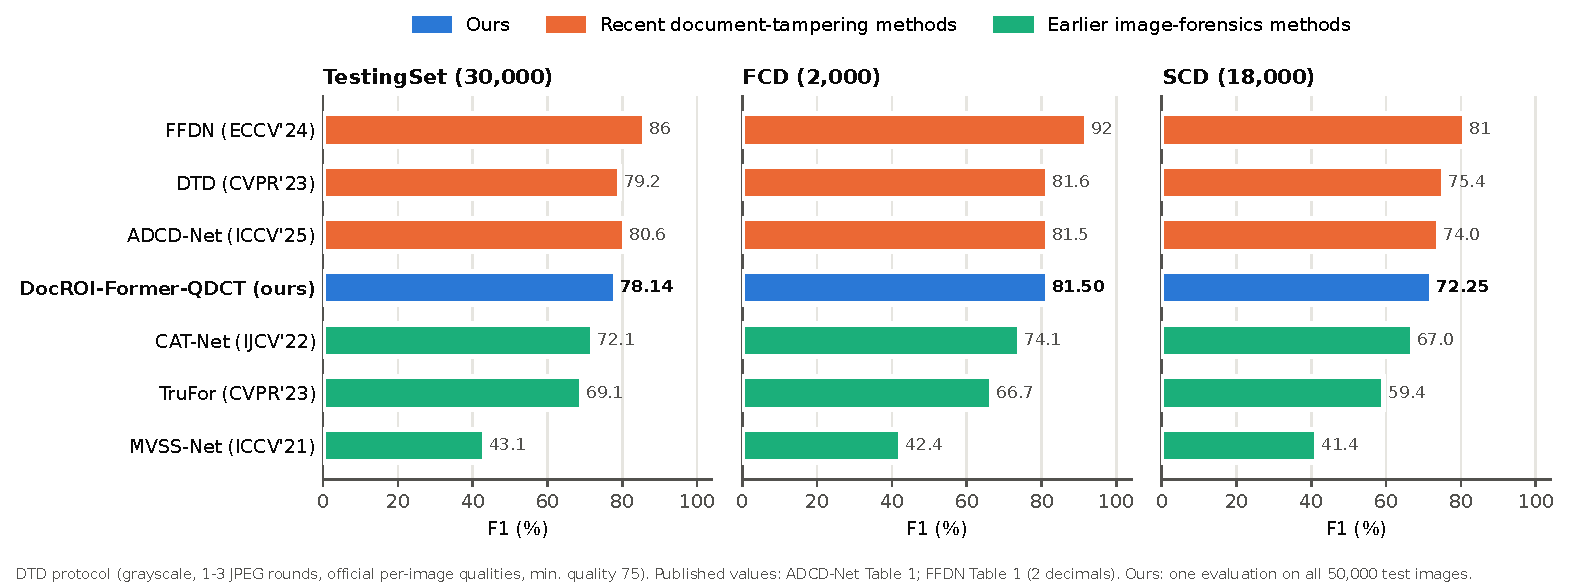
\includegraphics[width=\textwidth]{fig_f1_comparison.pdf}
\caption{F1 per test split under the DTD protocol ($q_{\min}=75$); sources as in
Table~\ref{tab:f1}. Bars start at zero.}
\label{fig:f1bars}
\end{figure}

\begin{figure}[!htbp]
\centering
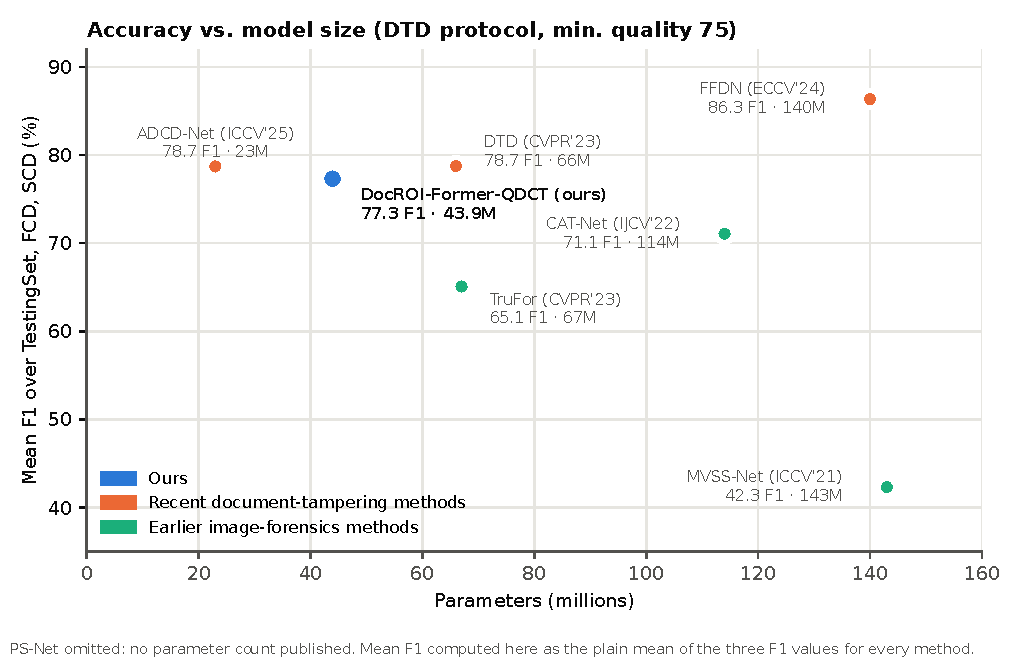
\includegraphics[width=0.74\textwidth]{fig_params_vs_f1.pdf}
\caption{Mean F1 over the three splits against parameter count (PS-Net omitted: no parameter
count published).}
\label{fig:params}
\end{figure}

\subsection{IoU against published methods}
Table~\ref{tab:iou} compares tampered-class IoU with the methods of DTD's Table~7. \ours\ is
second on TestingSet (77.3, behind DTD's 83.0) and SCD (60.3, behind 69.0), and third on FCD
(59.0, behind DTD's 75.0 and CAT-Net + CLTD's 60.0). The gap to DTD is larger in IoU than in F1,
most visibly on FCD, where F1 ties DTD but IoU is 16.0 lower. Section~\ref{sec:analysis} traces
this to false-positive pixels around larger edits.

\begin{table}[!htbp]
\centering
\caption{Tampered-class IoU (\%) under the DTD protocol ($Q=75$). Baselines: DTD~\cite{dtd}
Table~7. ADCD-Net and FFDN publish no tampered-class IoU.}
\label{tab:iou}
\begin{tabular}{@{}lcccc@{}}
\toprule
Method & TestingSet & FCD & SCD & Mean \\
\midrule
ManTra-Net~\cite{mantra}          & 18.0 & 17.0 & 16.0 & 17.0 \\
PSCC-Net~\cite{pscc}              & 17.0 & 16.0 & 19.0 & 17.3 \\
MVSS-Net~\cite{mvss}              & 43.0 & 41.0 & 40.0 & 41.3 \\
BEiT-Uper~\cite{beit,upernet}     & 59.0 & 35.0 & 34.0 & 42.7 \\
Swin-Uper~\cite{swin,upernet}     & 70.0 & 41.0 & 51.0 & 54.0 \\
CAT-Net~\cite{catnet}             & 74.0 & 42.0 & 55.0 & 57.0 \\
CAT-Net + CLTD~\cite{catnet,dtd}  & 71.0 & 60.0 & 54.0 & 61.7 \\
DTD~\cite{dtd}                    & \best{83.0} & \best{75.0} & \best{69.0} & \best{75.7} \\
\midrule
\textbf{\ours\ (ours)}            & 77.31 & 59.04 & 60.32 & 65.56 \\
\bottomrule
\end{tabular}
\end{table}

\subsection{Full metrics}
Table~\ref{tab:full} lists all metrics of the single evaluation run.

\begin{table}[!htbp]
\centering
\caption{Full metrics of \ours\ (one evaluation, all test images). P, R, F1 follow DTD's formula;
IoU is tampered-class IoU pooled over the split; mIoU is the two-class mean IoU.}
\label{tab:full}
\begin{tabular}{@{}lrccccc@{}}
\toprule
Split & $N$ & Precision & Recall & F1 & IoU & mIoU \\
\midrule
TestingSet & 30{,}000 & 79.20 & 77.10 & 78.14 & 77.31 & 88.49 \\
FCD        &  2{,}000 & 81.45 & 81.55 & 81.50 & 59.04 & 78.49 \\
SCD        & 18{,}000 & 69.97 & 74.68 & 72.25 & 60.32 & 79.94 \\
\bottomrule
\end{tabular}
\end{table}

\subsection{Per-split comparison and improvement over our previous model}
Figures~\ref{fig:test}--\ref{fig:scd} show F1 and IoU per split against the published methods and
against our previous model (\texttt{pguoctv3}), re-evaluated under the same protocol. That model
was trained at $384\times384$ in colour, with a floating-point DCT branch and no compression-aware
training, and was evaluated at 384\,px. It scored 56.9 / 52.9 / 50.0 F1 and 57.4 / 27.4 / 38.1
IoU. \ours\ improves on it by +21.2 / +28.6 / +22.2 F1 and +19.9 / +31.6 / +22.3 IoU. Because the
two models differ in several factors at once (resolution, colour, DCT branch, training
degradations, QK-norm), this gap is not an ablation of any single component.

\begin{figure}[!htbp]
\centering
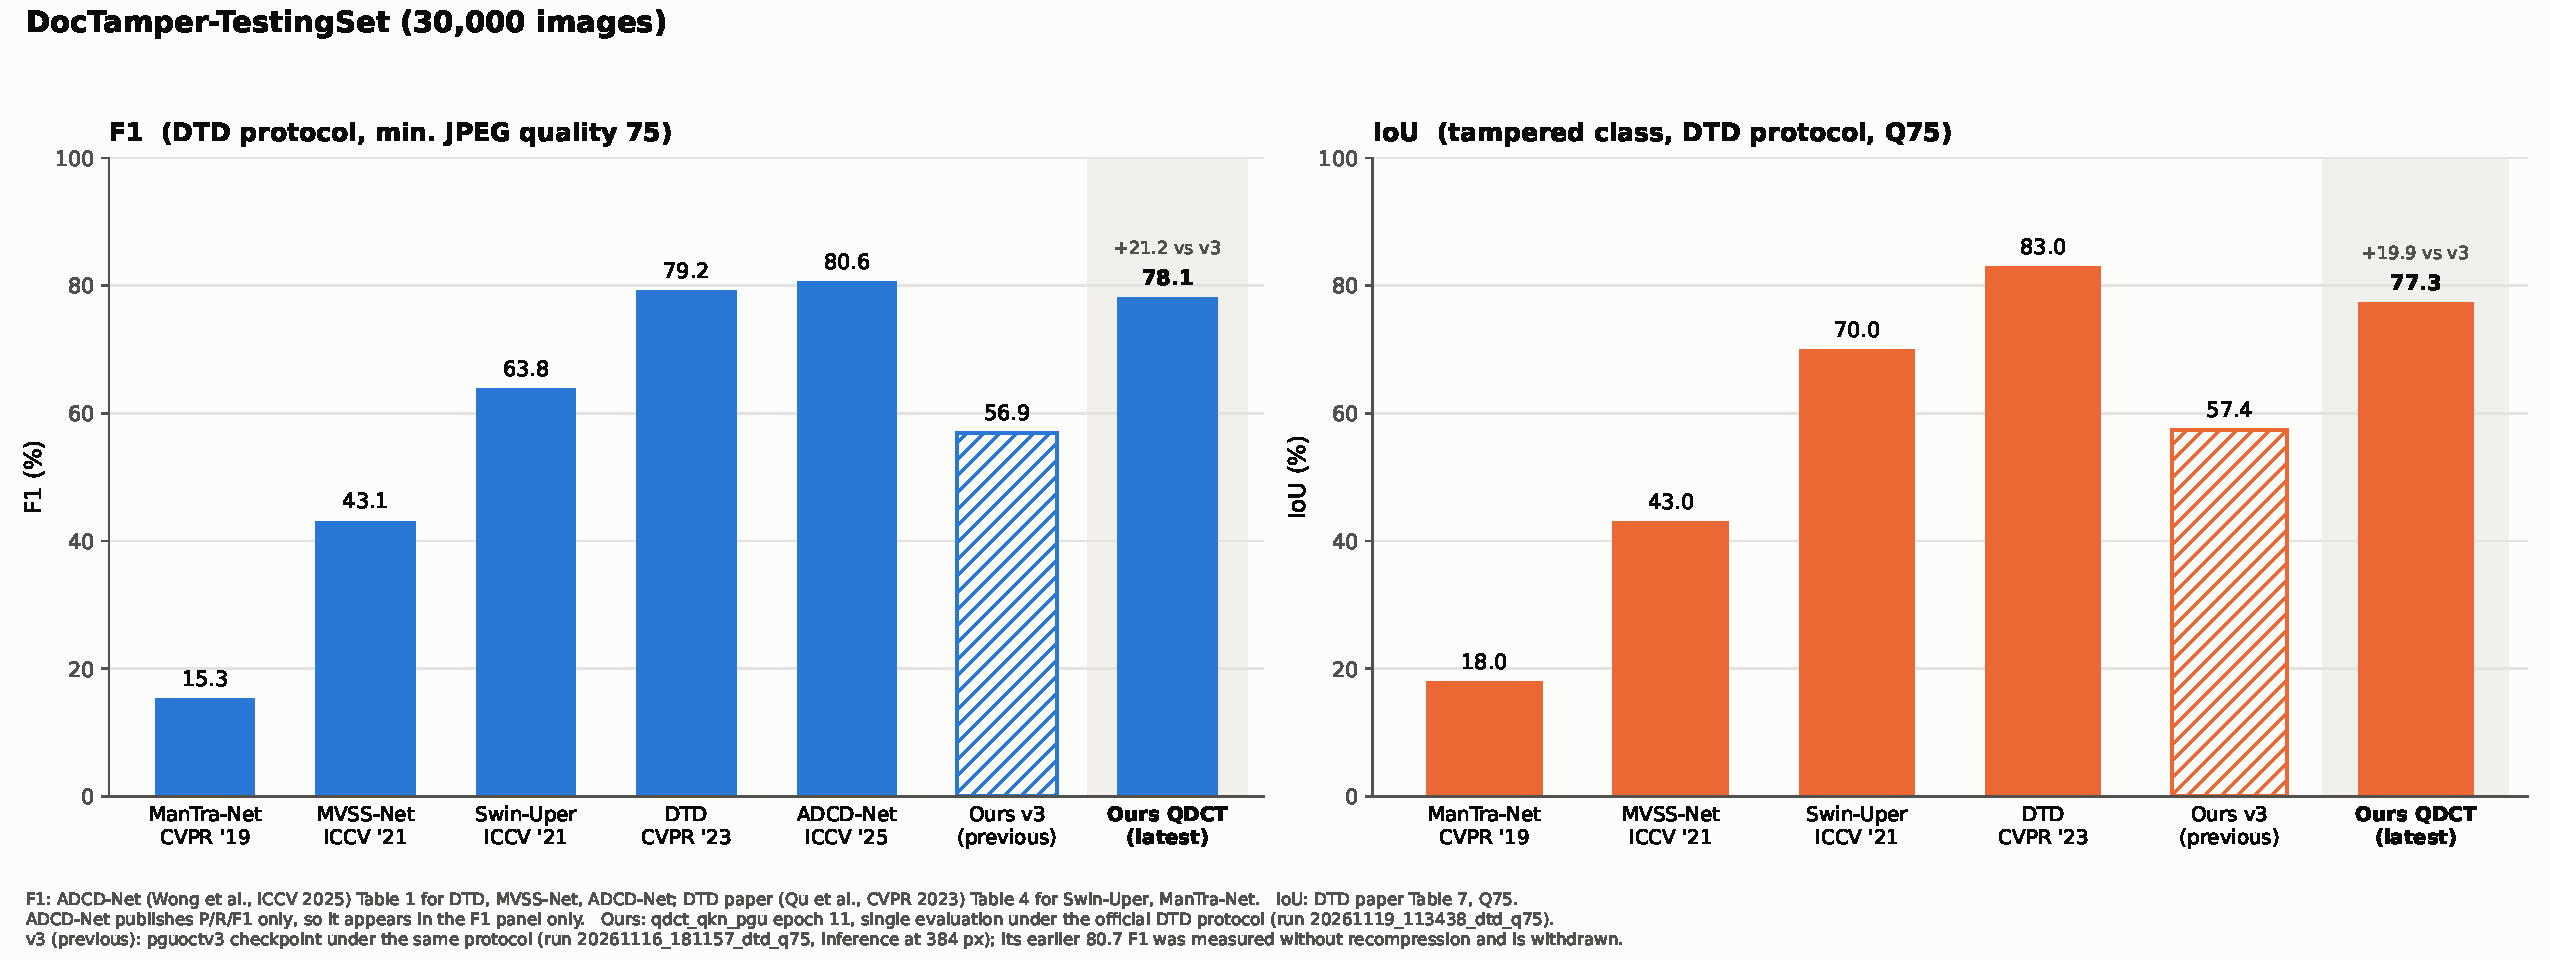
\includegraphics[width=\textwidth]{fig_testingset_f1_iou.pdf}
\caption{DocTamper-TestingSet: F1 (left) and IoU (right). The hatched bar is our previous model
under the same protocol. ADCD-Net is omitted from the IoU panel because it publishes no IoU.}
\label{fig:test}
\end{figure}

\begin{figure}[!htbp]
\centering
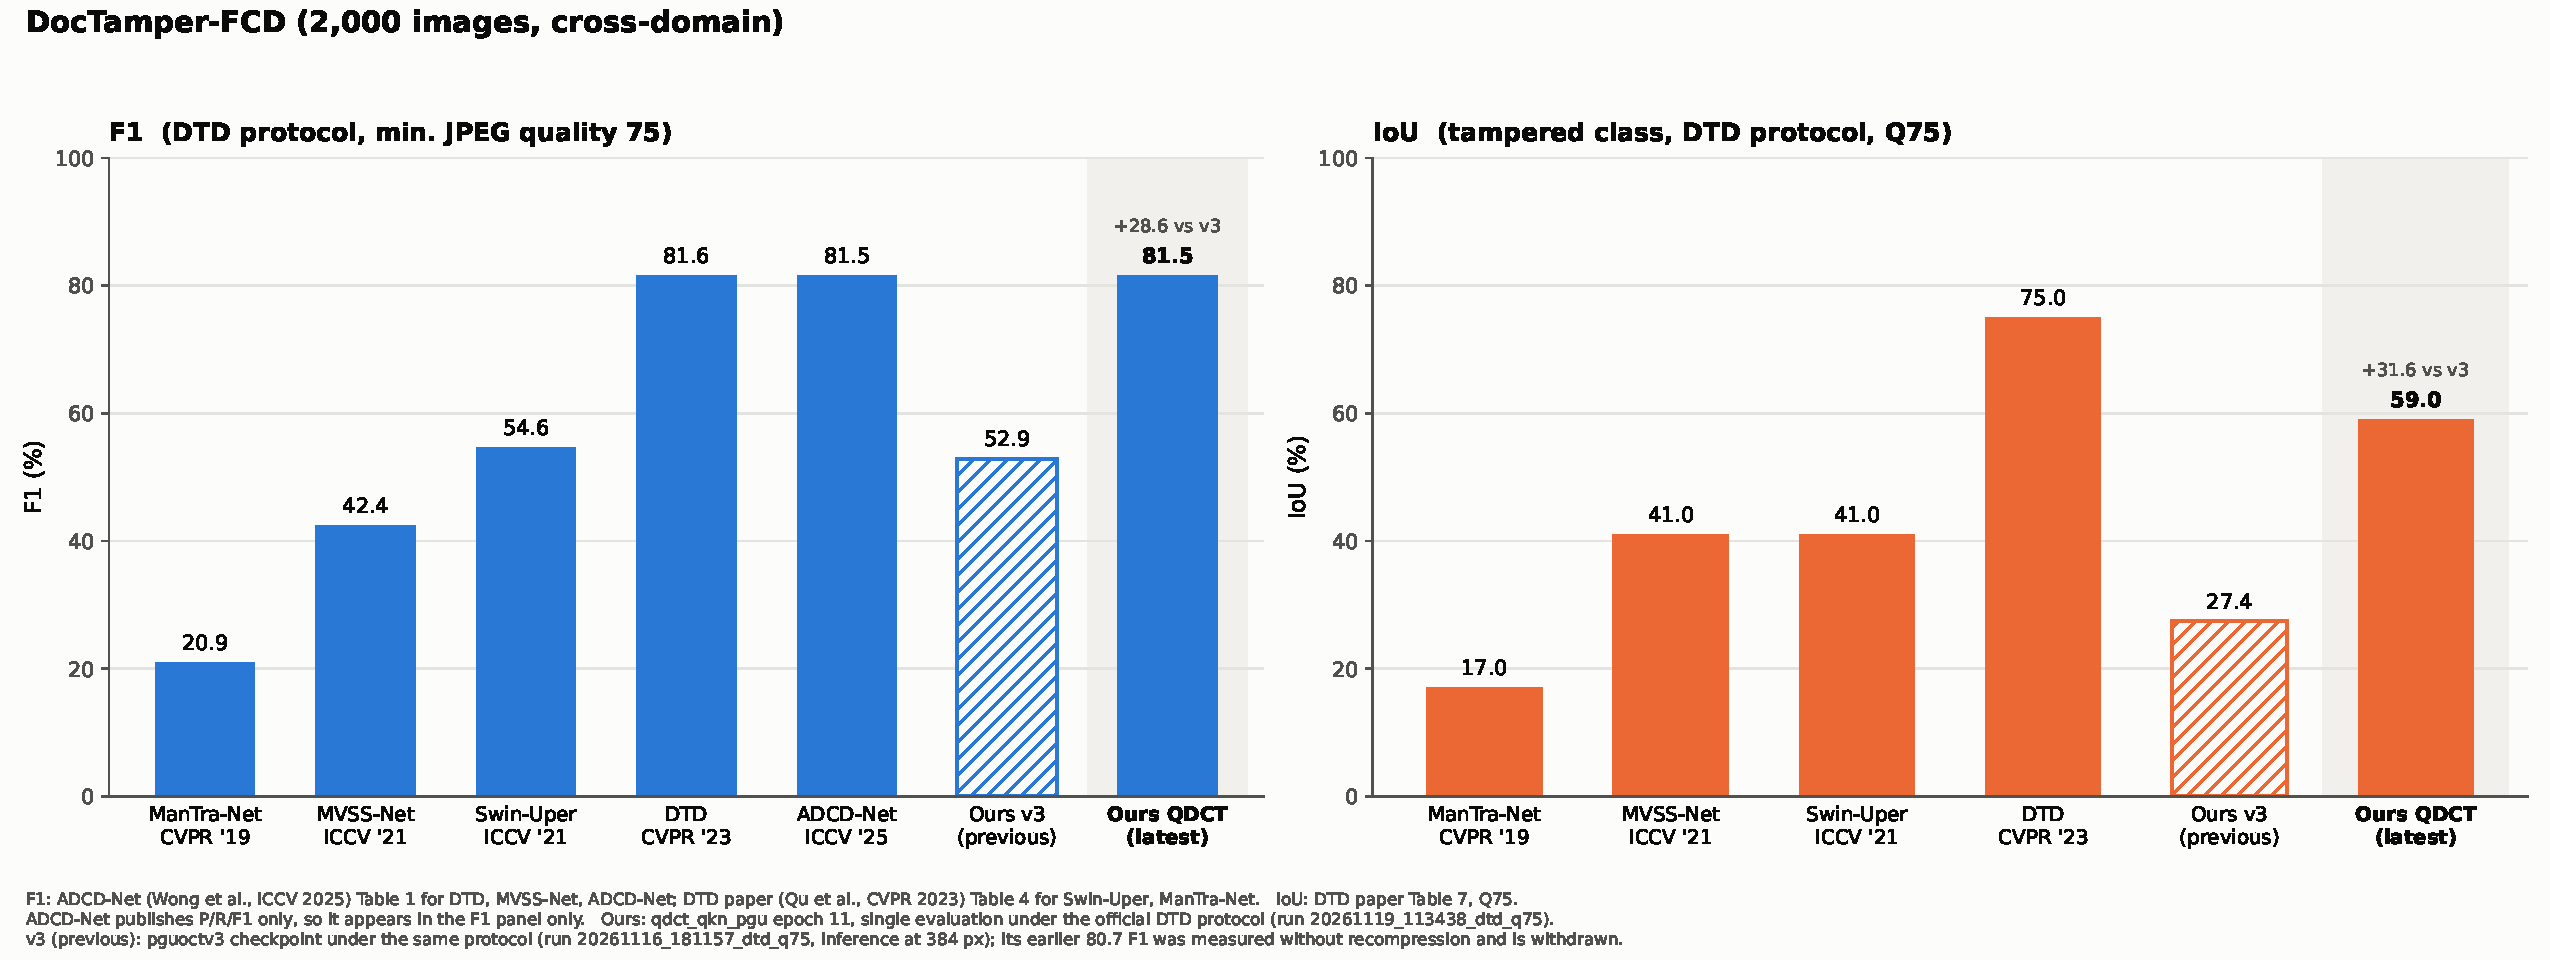
\includegraphics[width=\textwidth]{fig_fcd_f1_iou.pdf}
\caption{DocTamper-FCD (cross-domain): F1 (left) and IoU (right).}
\label{fig:fcd}
\end{figure}

\begin{figure}[!htbp]
\centering
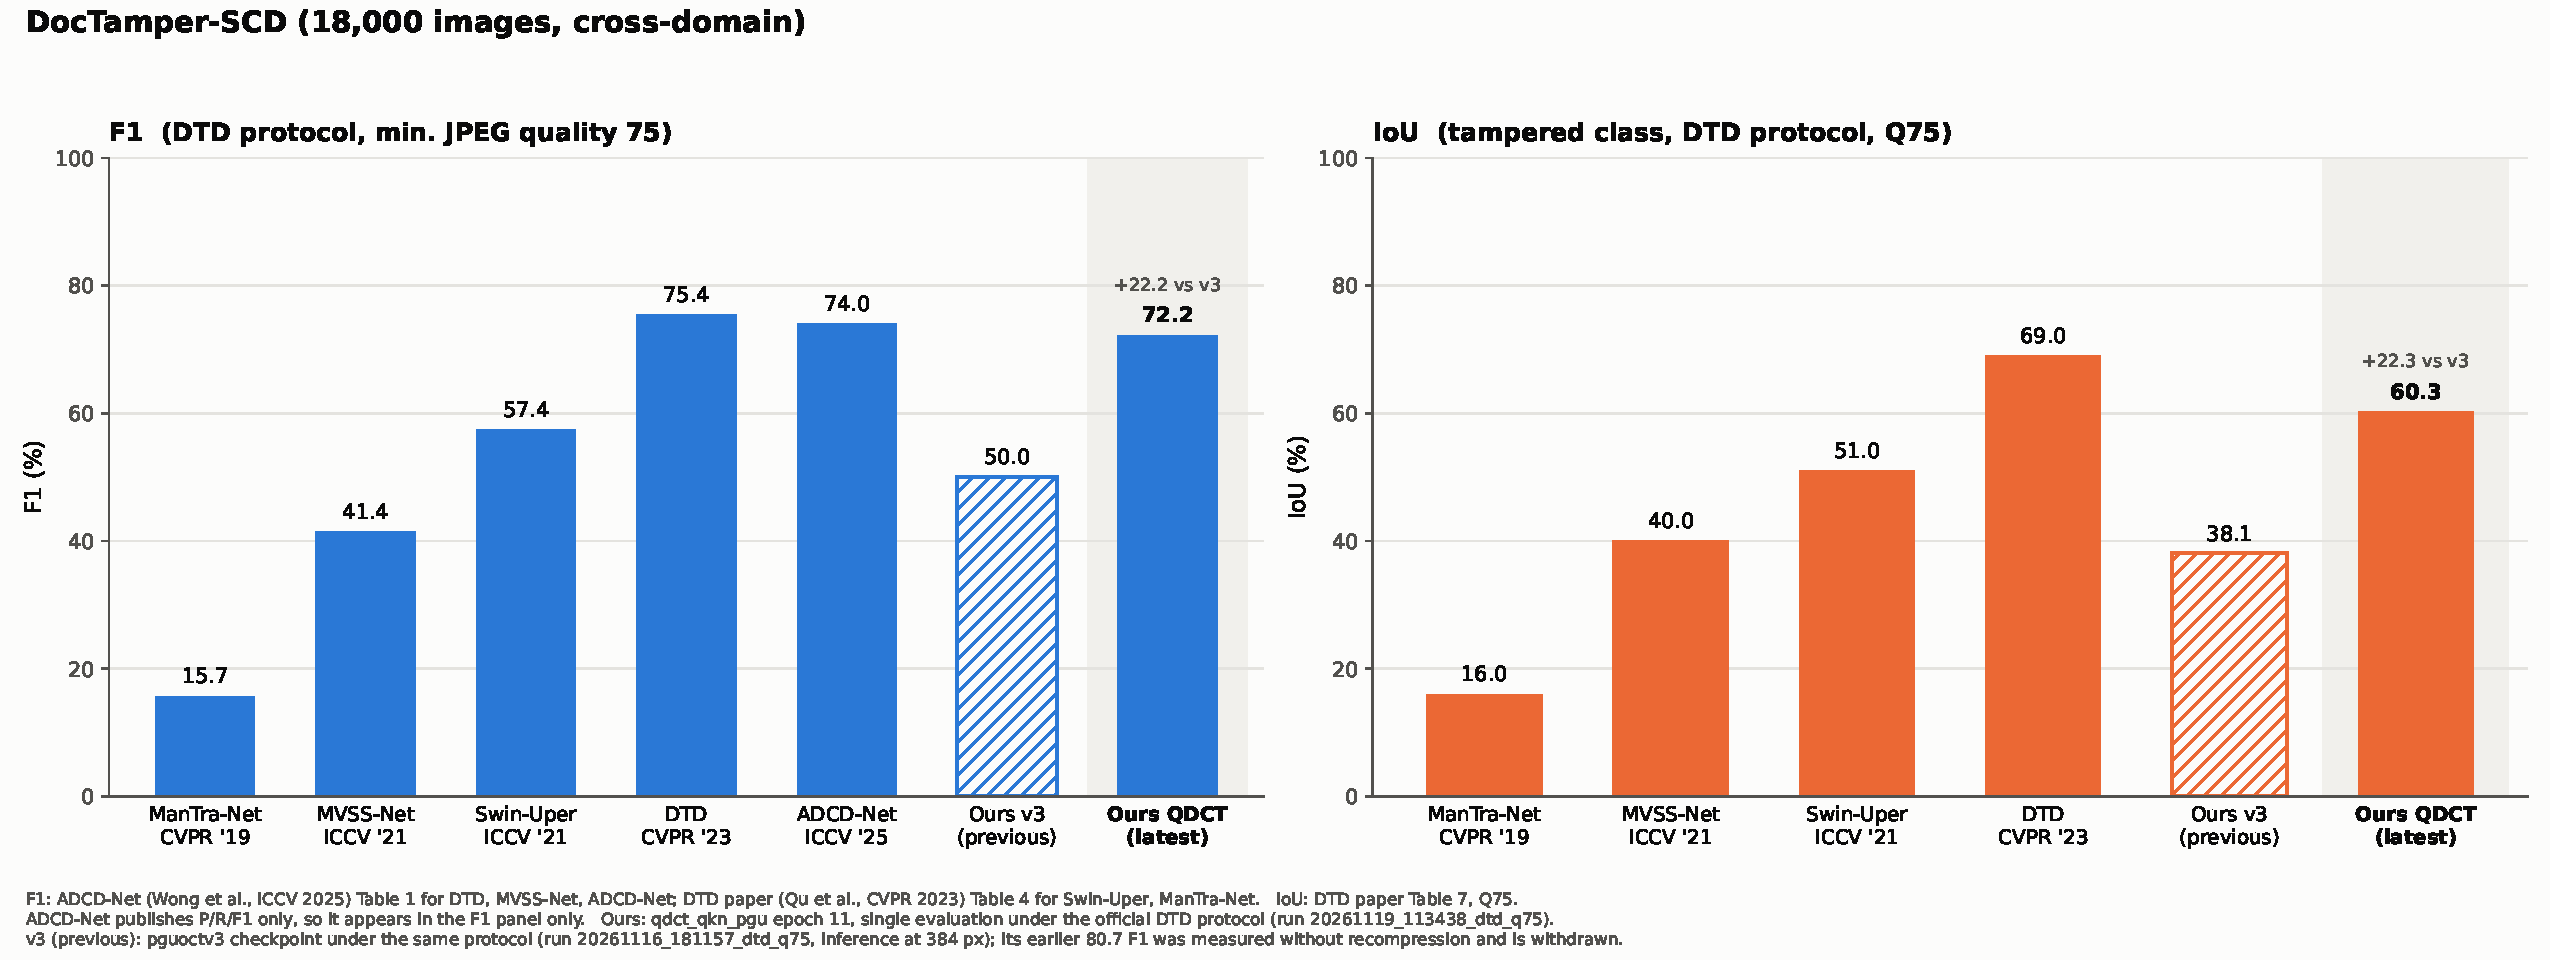
\includegraphics[width=\textwidth]{fig_scd_f1_iou.pdf}
\caption{DocTamper-SCD (cross-domain): F1 (left) and IoU (right).}
\label{fig:scd}
\end{figure}

% =====================================================================================
\section{Analysis}\label{sec:analysis}

\subsection{Where the points are lost}
Table~\ref{tab:breakdown} breaks F1 down by the tampered fraction of the image and by the number
of JPEG rounds, recomputed from the 50{,}000 per-image records.

\begin{table}[!htbp]
\centering
\caption{F1 (DTD formula) by tampered-area fraction and by number of JPEG rounds. Image counts in
parentheses. Images with $\geq$15\% tampered area are omitted (15 in TestingSet, 0 in FCD, 2 in
SCD).}
\label{tab:breakdown}
\small
\begin{tabular}{@{}lccc|ccc@{}}
\toprule
 & \multicolumn{3}{c|}{Tampered area / image} & \multicolumn{3}{c}{JPEG rounds} \\
Split & $<$1\% & 1--5\% & 5--15\% & 1 & 2 & 3 \\
\midrule
TestingSet & 70.4 (18{,}538) & 90.1 (10{,}489) & 96.3 (958) & 80.6 & 78.4 & 75.3 \\
FCD        & 68.1 (224)      & 83.6 (1{,}292)  & 81.8 (484) & 82.9 & 81.5 & 80.1 \\
SCD        & 69.0 (12{,}511) & 79.0 (5{,}295)  & 83.1 (192) & 73.9 & 71.9 & 71.0 \\
\bottomrule
\end{tabular}
\end{table}

\begin{itemize}
  \item \textbf{Small edits drive the gap.} Regions above 1\% of the image are localised well
        (90.1--96.3 F1 on TestingSet). Edits below 1\%, typically a single character, score
        about 70 F1 and make up 62\% of TestingSet and 70\% of SCD. In 10.3\% of TestingSet
        images no tampered pixel is detected. This is where the deficit to DTD and ADCD-Net
        comes from.
  \item \textbf{Compression is handled well.} From one to three JPEG rounds, F1 drops by 5.3 on
        TestingSet, 2.8 on FCD and 2.9 on SCD.
  \item \textbf{IoU on FCD is limited by false positives.} Pooled over all pixels, precision /
        recall are 86.6 / 87.8 on TestingSet but 68.5 / 81.0 on FCD, where the model predicts
        18\% more tampered pixels than exist. FCD's edits are larger on average (3.6\% of the
        image against 1.2\% on TestingSet), so over-segmentation around them dominates the
        pooled IoU while barely affecting the per-image F1. Tighter boundaries on large
        cross-domain edits would raise FCD IoU substantially.
\end{itemize}

\subsection{Training dynamics and generalisation}
Table~\ref{tab:val} shows the held-out validation F1 per epoch (from the training log). Validation
F1 of the selected epoch (76.8) and TestingSet F1 (78.1) agree, which is consistent with the
absence of selection leakage.

\begin{table}[!htbp]
\centering
\caption{Held-out validation F1 (2{,}500 training-set images, own fixed degradation table,
$q_{\min}=75$). The test sets were not used for any choice.}
\label{tab:val}
\begin{tabular}{@{}lcccccccccc@{}}
\toprule
Epoch & 1 & 2 & 3 & 4 & 6 & 8 & 9 & 10 & \textbf{11} & 12 \\
\midrule
Val F1 & 40.1 & 52.5 & 62.9 & 68.7 & 73.3 & 75.5 & 75.8 & 76.6 & \best{76.8} & 76.8 \\
Train $q_{\min}$ & 95 & 92 & 88 & 85 & 78 & 75 & 75 & 75 & 75 & 75 \\
\bottomrule
\end{tabular}
\end{table}

\subsection{Stability of cross-modal attention (N3)}\label{sec:stability}
An earlier run of the same architecture without QK-normalisation reached validation F1 66.5 at
epoch 4 and diverged in epoch 5 (gradient norm $\sim10^{13}$). We reconstructed the seeded data
order and replayed the failing batches: the attention logits at stages 3--4, where keys receive no
LayerNorm ($r_i=1$), had grown to a maximum magnitude of 157 and 97, against 5 and 23 at stages
1--2. With QK-normalisation all 88{,}125 updates were finite and the gradient norm stayed between
about 4.7 and 5.4. Before the divergence the two runs tracked each other closely (epochs 1--2:
40.9 / 53.0 without against 40.1 / 52.5 with QK-norm), so the fix restores stability without
changing the learning trajectory.

% =====================================================================================
\section{Integrity and reproducibility}\label{sec:audit}

\subsection{Rules enforced in code}
\begin{itemize}
  \item The trainer opens only the TrainingSet (asserted on the data path) and never reads DTD's
        test quality tables; training qualities come from our own generator.
  \item Model selection uses the 2{,}500 held-out training images only.
  \item The selected checkpoint was evaluated once: no threshold tuning, re-runs or test-time
        augmentation.
  \item \texttt{summary.csv} stores the SHA-256 of the checkpoint and of each quality table, and
        every test image has a row in a per-image CSV (50{,}000 rows).
\end{itemize}

\subsection{Independent audit of the evaluation records}
Because the headline numbers come from a single run, we audited the released records and the
evaluation code (23 November 2026). All checks passed.
\begin{enumerate}
  \item \textbf{Code review.} The evaluator contains no hard-coded results; it computes P, R, F1
        and IoU from the predicted and ground-truth masks. The model receives only the compressed
        image, the Otsu prior computed from that image, and the JPEG's luma plane and quantisation
        table. The ground-truth mask never enters the model. All images are scored in order,
        with no filtering.
  \item \textbf{Recomputation.} All twelve headline numbers (P, R, F1 and IoU on three splits)
        were recomputed exactly from the integer counts (ground-truth, predicted and true-positive
        pixels) in the per-image records, and every one of the 50{,}000 rows is arithmetically
        consistent ($\mathrm{tp}\le\min(\mathrm{gt},\mathrm{pred})$; P, R, F1, IoU follow from the
        counts).
  \item \textbf{Ground truth.} For every one of the 48{,}000 TestingSet and SCD images, the
        recorded number of ground-truth pixels equals the number of tampered pixels in the
        corresponding DocTamper label mask (FCD could not be checked: its data were not on the
        audit machine).
  \item \textbf{Protocol.} The SHA-256 of the three quality tables used equals that of DTD's public
        files, and for all 50{,}000 images the recorded JPEG quality sequence equals DTD's table
        entry, in DTD's order.
  \item \textbf{Live logging.} All 33 intermediate progress lines of \texttt{eval.log} equal the
        running metrics recomputed from the per-image CSV at the same sample count, and the log
        timestamps match the reported wall times.
  \item \textbf{Provenance.} The six record files were committed once, about four hours after the
        run, and never modified.
  \item \textbf{Anomalies explained.} Ten pairs of identical result rows in TestingSet correspond
        to ten pairs of byte-identical image and mask entries in the DocTamper TestingSet itself.
  \item \textbf{Standalone code.} The released code builds the exact configuration and runs a
        forward pass at $512\times512$ with 43.939M trainable parameters.
\end{enumerate}
\noindent What the audit cannot establish without the checkpoint is the predictions themselves.
Re-running the evaluator on a few hundred images with the fingerprinted checkpoint and comparing
the per-image rows closes this gap. The training-side figures (validation curve, divergence
diagnosis, run times) come from the training logs and were not part of the audit.

\subsection{Reproducibility record}
\begin{itemize}
  \item \textbf{Checkpoint} (epoch 11): \texttt{best\_docroi\_former\_qdct\_qdct\_qkn\_pgu.pth}\\
        SHA-256 {\footnotesize\texttt{76810b6110bf1d42e93247f0f592c346b4740be183f6861561f8e2edba5f0563}}
  \item \textbf{Quality tables} (SHA-256 prefixes; full values in \texttt{summary.json}):
        TestingSet \texttt{b34d4b52\dots}, FCD \texttt{db67bd20\dots}, SCD \texttt{3ddad77c\dots}
  \item \textbf{Evaluation record:} run \texttt{20261119\_113438\_dtd\_q75}, folder\\
        \texttt{reports/dtd\_protocol/FINAL\_RESULT\_ALLTHREELOGGED\_RESULT/}\\
        (\texttt{eval.log}, \texttt{summary.csv}, \texttt{summary.json}, one per-image CSV per split).
  \item \textbf{Environment:} PyTorch 2.12 (dev build, CUDA 12.8), one NVIDIA RTX 5080; GPU time
        about 99--105\,ms per image at batch 16.
\end{itemize}
Training and evaluation commands:
{\footnotesize
\begin{verbatim}
python train_academic.py --run_name qdct_qkn_pgu --init imagenet --resolution 512 \
    --epochs 12 --batch_size 4 --grad_accum 4 --dct quantized --qk_norm 1 --seed 0

python evaluate_dtd_protocol.py --checkpoint <ckpt> --infer_size 0 \
    --datasets TestingSet,FCD,SCD --minq 75 --threshold 0.5
\end{verbatim}
}

% =====================================================================================
\section{Limitations and future work}\label{sec:limits}
\begin{enumerate}
  \item \textbf{No component ablations.} N1, N2, N4 and N5 are supported only by the full-system
        result. The planned ablations retrain the same recipe with one change each: no routing
        ($\rho\equiv1$, $m\equiv1$); no quantised-DCT stream, or no FiLM conditioning; plain
        bilinear decoding from stride 4 instead of the PGU head; and $\lambda_{\mathrm{font}}=0$.
  \item \textbf{Single run, single seed.} There are no error bars; the compared papers also report
        single runs. Repeating the final recipe with three seeds would bound the variance.
  \item \textbf{Re-implemented protocol.} The evaluator follows DTD's script step by step and uses
        DTD's exact tables, but it has not yet been validated by reproducing a published number
        with DTD's released weights.
  \item \textbf{Small edits.} F1 is about 70 on regions below 1\% of the image, which accounts for
        most of the gap to the state of the art. Directions include stronger supervision at
        stride 2 and full resolution for tiny regions, region-size-aware loss weighting, and
        character-level context.
  \item \textbf{Boundary over-segmentation on FCD.} Pooled precision of 68.5 limits IoU on
        large cross-domain edits.
  \item \textbf{Auxiliary heads.} Almost every DocTamper training image contains tampering, so the
        global head is effectively untrained on authentic documents and must not be used as a
        document classifier.
  \item \textbf{Domain.} DocTamper is predominantly Chinese-language documents. Behaviour on other
        document types, and the false-alarm rate on authentic documents, have not been measured
        for this checkpoint.
\end{enumerate}

% =====================================================================================
\section{Conclusion}\label{sec:conclusion}
\ours\ localises tampered text in recompressed document images by letting the RGB stream query
forensic evidence (residuals plus exact, quantisation-conditioned DCT coefficients) only at
document content, with stabilised cross-modal attention and a thin-region decoder. Evaluated once
under the official DTD protocol, it reaches 78.1 / 81.5 / 72.3 F1 and 77.3 / 59.0 / 60.3 IoU on
TestingSet / FCD / SCD with 43.9M parameters. It ties ADCD-Net and nearly matches DTD on the
cross-domain FCD split and improves on our previous model by more than 20 F1 on every split, but
it is not state of the art: it trails DTD and ADCD-Net by 1--3 F1 on TestingSet and SCD and FFDN by
8--11. The error analysis points to two concrete targets, edits below 1\% of the image and
boundary precision on large cross-domain edits, and the ablations listed above are needed before
the individual components can be claimed as contributions.

% =====================================================================================
\begin{thebibliography}{99}\small
\bibitem{dtd} C.~Qu, C.~Liu, Y.~Liu, X.~Chen, D.~Peng, F.~Guo and L.~Jin, ``Towards robust
  tampered text detection in document image: New dataset and new solution,'' in \emph{CVPR},
  2023.
\bibitem{ffdn} Z.~Chen \emph{et al.}, ``Enhancing tampered text detection through frequency
  feature fusion and decomposition,'' in \emph{ECCV}, 2024.
\bibitem{adcd} K.~Wong \emph{et al.}, ``ADCD-Net: Robust document image forgery localization
  via adaptive DCT feature and hierarchical content disentanglement,'' in \emph{ICCV}, 2025.
\bibitem{mantra} Y.~Wu, W.~AbdAlmageed and P.~Natarajan, ``ManTra-Net: Manipulation tracing
  network for detection and localization of image forgeries with anomalous features,'' in
  \emph{CVPR}, 2019.
\bibitem{mvss} X.~Chen \emph{et al.}, ``Image manipulation detection by multi-view
  multi-scale supervision,'' in \emph{ICCV}, 2021.
\bibitem{pscc} X.~Liu \emph{et al.}, ``PSCC-Net: Progressive spatio-channel correlation network
  for image manipulation detection and localization,'' \emph{IEEE TCSVT}, 2022.
\bibitem{catnet} M.-J.~Kwon \emph{et al.}, ``Learning JPEG compression artifacts for image
  manipulation detection and localization,'' \emph{IJCV}, 2022.
\bibitem{trufor} F.~Guillaro \emph{et al.}, ``TruFor: Leveraging all-round clues for
  trustworthy image forgery detection and localization,'' in \emph{CVPR}, 2023.
\bibitem{swin} Z.~Liu \emph{et al.}, ``Swin Transformer: Hierarchical vision transformer using
  shifted windows,'' in \emph{ICCV}, 2021.
\bibitem{beit} H.~Bao, L.~Dong, S.~Piao and F.~Wei, ``BEiT: BERT pre-training of image
  transformers,'' in \emph{ICLR}, 2022.
\bibitem{upernet} T.~Xiao \emph{et al.}, ``Unified perceptual parsing for scene understanding,''
  in \emph{ECCV}, 2018.
\bibitem{pvtv2} W.~Wang \emph{et al.}, ``PVT v2: Improved baselines with pyramid vision
  transformer,'' \emph{Computational Visual Media}, 2022.
\bibitem{bayar} B.~Bayar and M.~C.~Stamm, ``Constrained convolutional neural networks: A new
  approach towards general purpose image manipulation detection,'' \emph{IEEE TIFS}, 2018.
\bibitem{srm} J.~Fridrich and J.~Kodovsk\'y, ``Rich models for steganalysis of digital
  images,'' \emph{IEEE TIFS}, 2012.
\bibitem{qknorm} M.~Dehghani \emph{et al.}, ``Scaling vision transformers to 22 billion
  parameters,'' in \emph{ICML}, 2023.
\bibitem{film} E.~Perez \emph{et al.}, ``FiLM: Visual reasoning with a general conditioning
  layer,'' in \emph{AAAI}, 2018.
\bibitem{focal} T.-Y.~Lin \emph{et al.}, ``Focal loss for dense object detection,'' in
  \emph{ICCV}, 2017.
\bibitem{boundary} H.~Kervadec \emph{et al.}, ``Boundary loss for highly unbalanced
  segmentation,'' in \emph{MIDL}, 2019.
\bibitem{infonce} A.~van den Oord, Y.~Li and O.~Vinyals, ``Representation learning with
  contrastive predictive coding,'' arXiv:1807.03748, 2018.
\end{thebibliography}

\end{document}
